\documentclass{standalone}
\usepackage{tikz}
\usepackage{ctex,siunitx}
\usepackage{tkz-euclide}
\usepackage{amsmath}
\usetikzlibrary{patterns, calc}
\usetikzlibrary {decorations.pathmorphing, decorations.pathreplacing, decorations.shapes,}
\begin{document}
\small
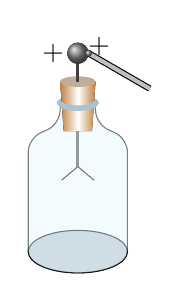
\begin{tikzpicture}[>=latex,scale=0.9]
  % \useasboundingbox(-1,-2)rectangle(8,6);
  \draw[very thick,darkgray](0,0)--(0,1.2);
  \draw(0,0)--(220:0.3)(0,0)--(320:0.3);
  \draw[fill=cyan!10!lightgray](0,-1.2)ellipse(0.7 and 0.3);
  \draw[rounded corners=5pt,fill=cyan!10,opacity=0.5](-0.7,-1.2)--(-0.7,0.4)--(-0.25,0.6)--(-0.25,1.0)--(0.25,1.0)--(0.25,0.6)--(0.7,0.4)--(0.7,-1.2);
  \draw[fill=cyan!10,opacity=0.5](0.7,-1.2)arc(360:180:0.7 and 0.3);
  \fill[cyan!20!lightgray,](0,0.9)ellipse(0.3 and 0.1);
  \fill[left color=brown,right color=brown,middle color=white](-0.20,0.5)--++(-0.05,0.7)--++(0.5,0)--++(-0.05,-0.7)--cycle;
  \fill[brown!30!lightgray](0,1.2)ellipse(0.25 and 0.075);
  \draw[very thick,darkgray](0,1.2)--(0,1.6);
  \fill[ball color=gray](0,1.6)circle(0.15);
  \draw[cyan!20!lightgray,line width=2pt](-0.25,0.9)arc(180:360:0.25 and 0.075);
  \node at (-0.35,1.6){$+$};
  \node at (0.3,1.7){$+$};
  \draw[double=gray!50,double distance=1.5pt](0.15,1.6)--++(-30:1);
  \fill[ball color=gray](0.15,1.6)circle(1.35pt);
  % \draw[double=cyan,double distance=3pt,opacity=0.5](0.3,1.0)arc(360:180:0.3 and 0.09);
\end{tikzpicture}
\end{document}